\documentclass[12pt]{article}
\usepackage{graphicx}
\usepackage{hyperref}
\usepackage{cite}
\usepackage{float} % for [H] anchoring method
\usepackage[top=1.4in, bottom=1.4in, left=1.4in, right=1.4in]{geometry}
\graphicspath{ {pngs/} }
\usepackage{mdframed}

\newcommand{\specialcell}[2][c]{%
	\begin{tabular}[#1]{@{}c@{}}#2\end{tabular}}

\begin{document}
\title{CSE326 Semester Project Design Spec: Anttris}
\author{Team \#5\\\\Chris Aikman\\Benji Cope\\Skyler Manzanares\\Hugo Rivera\\Sean Turner}
\maketitle

\section{Project Overview} % CA
Anttris is a unique and competitive three-dimensional puzzle game that can be played alone or against others online. The core of Anttris' gameplay lies in solving various puzzle cubes that are composed of blocks. These puzzles vary from simple to complicated and require critical thinking to complete. Players solve these puzzle cubes by interacting with individual blocks until they are all destroyed.

Anttris includes two different game modes: single-player and competitive. Single-player focuses on clearing puzzles with an emphasis placed on efficiency of the solution which is measured by the amount of moves and total time. Competitive games shifts the focus to solving cubes faster than an opponent.

While the two core game modes provide a fun and unique game, Anttris really shines when it comes to the ability to create your own puzzles through a built-in editor. Players are also able to use the puzzles they created when playing competitively. The goal of the game is expanded from simply solving a cube faster than your opponent to \textsl{creating} a puzzle that will challenge your opponent while you solve their puzzle first.
\subsection{Scope and Objectives} %CA / HR
While Anttris is a simple puzzle game, it was designed to be extendable. The core scope of the game involves creating working self-contained executables for many different platforms which include, but are not limited to, PC, Max and Linux. These executables will at the very least contain single-player and competitive online games modes with a working editor. To do this, we are utilizing a game development framework called Godot \cite{godot:gameengine} that provides the basic functionality of a three-dimensional game. A mixture of networking libraries and Godot's networking features will be utilized to complete the competitive game mode which will be done using a peer-to-peer direct connection. Puzzles will be both hand crafted and generated using a custom puzzle generator. To ensure that puzzles created in the editor are solvable, the game will also include a puzzle solver that will quickly and efficiently determine if a generated or editor-created puzzle can be solved.

To further extend the scope, Anttris may include several other features if time permits. These features may include an online server, non-block-shaped puzzles, game result statistics, hiscore list and replay mode. A main server will allow users to randomly connect to opponents instead of using direct connection. Non-block-shaped puzzles will allow for more creative freedom in the editor and give puzzles a fun look. Game result statistics will show how the game played out with a graph of time versus blocks left for the user and their component. A hiscore list will let users see where they rank among their competition throughout the world. Finally, a replay mode will let the user watch a single-player or competitive game, allowing them to see where they need to improve or get tips from opponents.

The main objectives of the project involve:
\begin{itemize}
 \item Completing core gameplay mechanics. This involves completing a single-player game that uses user input to manipulate the game's state into winning the game.
 \item Completing graphical elements. This involves creating and modifying the visual elements of the game from the textures of the 3d objects to the graphical user interface.
 \item Completing multiplayer gameplay mechanics. This involves connecting two individual players on separate machines in order for the players to compete with each other on preset puzzles or puzzles they have made themselves.
 \item Completing a puzzle generator. This involves creating an efficient way of generating unique puzzles that are both fun and solveable with varying levels of difficulty.
 \item Completing a puzzle solver. This involves creating an efficient way of solving any puzzle, generated or editor-created.
 \item Adding additional gameplay mechanics. This involves adding on additional features that we may not have enough time to complete within the project's timeline, but would like to if the base project is completed before scheduled. These ideas involve:
  \begin{itemize}
  \item Adding online connections through a client-server setup instead of through peer-to-peer connections.
  \item Adding new competitive and single player game modes based on the same puzzle mechanics, such as �race the clock' or �remove all blocks'.
  \item Adding puzzles that are not cube shaped.
  \item Adding a hiscore board.
  \item Adding replays.
  \end{itemize}
\end{itemize}
\subsection{Supplementary Requirements} % CA
\subsubsection{Interface Requirements}
In Anttris, the user interface is made to be simple and intuitive so that any user will be able to quickly pick up the game and play. Menus are clear and simple and the in-game user interface is minimal so that the user can focus on gameplay. The editor follows these same rules by providing maximum functionality with the least amount of visual clutter.

Standard input methods will be used depending on the device. A standard mouse on a personal computer will cover all of the games input requirements while a touch screen will be supported on mobile devices. A keyboard (on screen or physical) will be used for text input that includes entering an IP address or entering the user's online display name.

\subsubsection{Performance Requirements}
Anttris will follow industry standards meaning that it needs to look visually pleasing and also run efficiently on all modern machines including common computers and mobile devices. Graphics will be professional, light and clean as usual for puzzle games. Anttris will deliver a minimum of 30 frames per second with a maximum of 60 frames per second depending on the device. Intended devices include personal computers commonly found in a traditional office space as well as modern smart phones that run on iOS or Android. Frame rates will be consistent and not choppy. Failing to meet either of these requirements is unacceptable.

\section{Customer Requirements}
% SM
\subsection{Use-Case Diagrams}
    \begin{figure}[H]
        \centering
        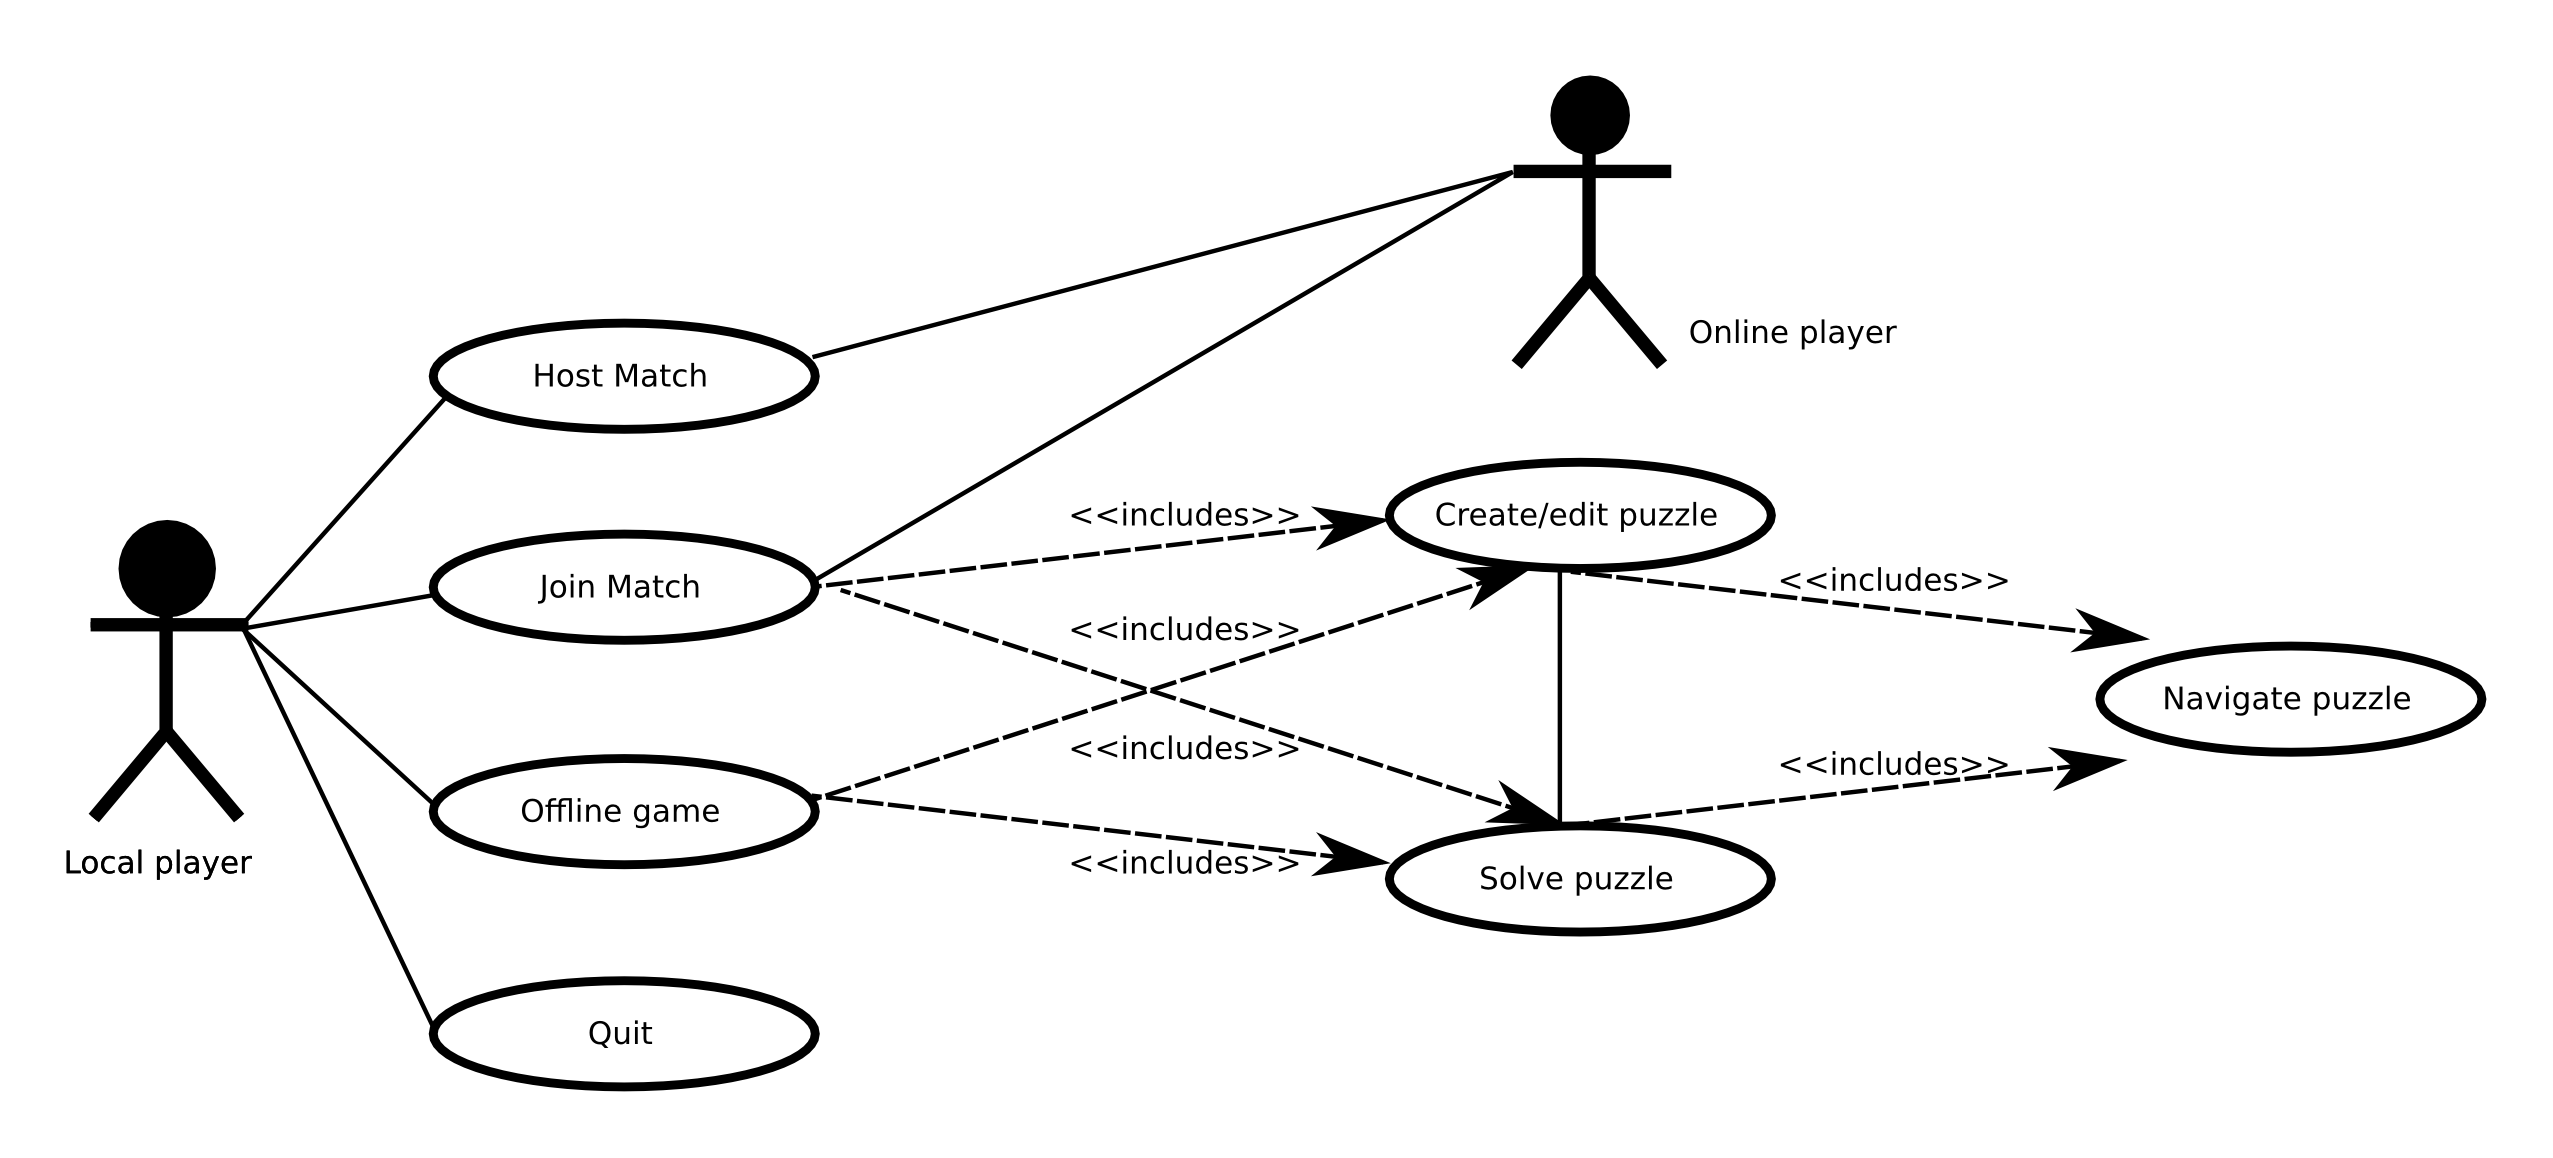
\includegraphics[width=6in]{use_cases.png}
        \caption{Use Case Diagram}
    \end{figure}

\subsection{Actor Descriptions}
    \begin{description}
        \item[Local player] is the local user and has full
            access to the mouse and keyboard or touchscreen interface.
        \item[Online player] is a non-local player. There is two-way
            communication between this type of player and the local player.
            There may be 0 or more online players.
        \item[The Host] has special powers, may disconnect other players and
            block players from selecting different puzzles. This player could
            be Local or Online.
    \end{description}

\subsection{Use-case Descriptions}
\begin{mdframed}
    \subsubsection{Host match}
    \begin{description}
        \item[Entry conditions] Internet connection.
        \item[Exit conditions] Will return to game menu. All players
            disconnected or all puzzles have been solved.
        \item[Participating Actors] Online player and local player.
        \item[Flow of events]:
            \begin{enumerate}
                \item The user presses the appropriate menu button.
                \item User creates a game, selects number of players and game
                    type
                \item User shares (friendly looking) match ID with other
                    players. These players may connect to the match
                \item Puzzle Selector appears.
                \item The user may configure the game with this screen.
                    This
                    entails choosing a puzzle and a game mode (edit or solve).
                    Other players can be prevented from making such
                    modifications.
                \item This Puzzle Selector will create a Puzzle Scene
                \item The scene will change from the main menu to the Puzzle
                    Scene.
                \item Additional view-ports will be added to the game screen. 
                These show the progress of online players in an interface
                similar to the local player's puzzle.

            \end{enumerate}
    \end{description}
\end{mdframed}

\begin{mdframed}
    \subsubsection{Join match}
    \begin{description}
        \item[Entry conditions] Internet connection. The menu must be present.
        \item[Exit conditions] Will return to game menu. All players
            disconnected or all puzzled have been solved.
        \item[Participating Actors] Online player and local player.
        \item[Flow of events]:
            \begin{enumerate}
                \item The user presses the appropriate menu button.
                \item Puzzle Selector appears.
                \item The user may configure the game with this screen, if
                    the game host allows it. This would
                    entail choosing a puzzle and a game mode (edit or solve).
                \item This Puzzle Selector will create a Puzzle Scene
                \item The scene will change from the main menu to the Puzzle
                    Scene.
                \item Additional view-ports will be added to the game screen. 
                These show the progress of online players in an interface
                similar to the local player's puzzle.
            \end{enumerate}
    \end{description}
\end{mdframed}


\begin{mdframed}
    \subsubsection{Offline game}
    \begin{description}
        \item[Entry conditions] Menu must be present.
        \item[Exit conditions] Will return to game menu. Puzzle has been
            solved.
        \item[Participating Actors] Local player.
        \item[Flow of events]:
            \begin{enumerate}
                \item User selects the appropriate menu button.
                \item Puzzle Selector appears.
                \item The user may configure the game with this screen. This
                    entails choosing a puzzle and a game mode (edit or solve).
                \item This Puzzle Selector will create a Puzzle Scene
                \item The scene will change from the main menu to the Puzzle
                    Scene.
            \end{enumerate}
    \end{description}
\end{mdframed}


\begin{mdframed}
    This use case includes the Host Match, Join Match and Offline Game
    use cases.
    \subsubsection{Edit puzzle}
    \begin{description}
        \item[Entry conditions] A Puzzle Scene must be loaded and edit mode
            must be activated.
        \item[Exit conditions] Will return to game menu. The puzzle may be
            saved to the disk.
        \item[Participating Actors] Online player or local player.
        \item[Flow of events]:
            \begin{enumerate}
                \item The user navigates the puzzle
                \item If a position on the grid is selected, the Block Modifier
                    is presented. This position may be empty or it may
                    contain a block.
                \item The user may change properties of the block using this
                    screen.
                \item Blocks may be added or removed using this same screen.
            \end{enumerate}
            Puzzle preview:
            \begin{enumerate}
                \item User may press the preview button
                \item The user will try the puzzle in Solve Puzzle mode until
                    that mode's exit conditions are met.
                    A special banner will graphically indicate preview mode.
                \item The solving scene will have a special button for
                    returning to the editing scene
            \end{enumerate}
    \end{description}
\end{mdframed}


\begin{mdframed}
    This use case includes the Host Match, Join Match and Offline Game
    use cases.
    \subsubsection{Solve puzzle}
    \begin{description}
        \item[Entry conditions] A Puzzle Scene must be loaded and solve mode
            must be activated.
        \item[Exit conditions] Will return to game menu or puzzle editor.
            If the game is over, an overview of results will be shown and the
            steps taken to solve the puzzle may be saved to the disk.
        \item[Participating Actors] Online player or local player.
        \item[Flow of events]:
            \begin{enumerate}
                \item The user navigates the puzzle
                \item If a block is selected, the block runs any associated
                    Block Action.
                \item These Block Actions may modify the block's properties or
                    request the addition or removal of blocks, including the
                    selected block, from the Grid Manager.
                \item This sequence is repeated until the winning block is
                    found, the user quits, or a losing condition is met.
                \item User's actions may be mirrored on an online player's
                    screen, likewise, separate Puzzle Scenes  may be updated
                    with any moves made by other players.
            \end{enumerate}
    \end{description}
\end{mdframed}


\begin{mdframed}
    \subsubsection{Navigate puzzle}
    This use case includes the Solve puzzle and Edit puzzle use cases.
    \begin{description}
        \item[Entry conditions] Puzzle scene loaded and permission to move.
            Input devices must be functional.
        \item[Exit conditions] The game must offer continuous feedback.
            If the entry conditions are met, any further input must be
            acted on as soon as possible.
        \item[Participating Actors] Online player and local player.
        \item[Flow of events]:
        	\\
            Camera motion:
            \begin{enumerate}
                \item User drags with a mouse or touchscreen
                \item The camera changes position
            \end{enumerate}

            Block selection:
            \begin{enumerate}
                \item User clicks with mouse or taps on touchscreen
                \item The 3D coordinates are translated into a position on
                    a game ``board.''
                \item The Grid Manager is notified of input and the grid
                    position.
                \item If a block is present there, it is selected and activated.
                    Exact actions depend on the game mode.
                \item If a block is not present, the space is selected. This
                    is only useful in edit mode.
                \item The user may end the game at any point through the pause
                    menu.
            \end{enumerate}

    \end{description}
\end{mdframed}


\begin{mdframed}
    \subsubsection{Quit}
    \begin{description}
        \item[Entry conditions] Game must be running. This action is
            asynchronous and may activate at any point.
        \item[Exit conditions] Game, be gone!
        \item[Participating Actors] Local player.
        \item[Flow of events]:
            \begin{enumerate}
                \item User presses the quit button on a menu
                \item or User presses appropriate sequence of keys, such as
                    the escape key or the alt and F4 combo.
                \item Some data may be saved, such as the puzzle being currently 
                edited.
                \item The program shuts down gracefully.
            \end{enumerate}
    \end{description}
\end{mdframed}



\section{Architectural Design}
% HR
\subsection{Subsystem Architecture}
% SM
\begin{figure}[H]
    \centering
    
\includegraphics[width=6in]{subsys_arch.png}
    \caption{Use Case Diagram}
\end{figure}
The two primary subsystems of Anttris are the puzzle-solving system and the online system.

The puzzle-solving system is composed generically over a puzzle viewer and attached event
handling that allows interaction with the puzzle. Both offline games and online ones use 
the puzzle viewer, as does the unique puzzle-editing mode. The puzzle viewer is used by
all three unique modes, and works with our 3D model interaction system to provide
interactivity. This system is built on the Godot 3d Engine, which uses OpenGL.

The online system breaks down immediately into host mode or remote client mode. The host 
mode interfaces with the application-generic session-host system, which works in conjunction
with the session lobby to facilitate remote clients to connect and play against the host. 
Remote clients also work closely with the session lobby to find hosts to play against. Both
the session lobby and the session-host system work with the Godot Online Subsystem to provide
connectivity. The Godot Online Subsystem is built over tcp-udp/ip.

\subsection{Deployment Model}
% HR
\section{Use Case Realization Design}
% HR, I did Use Cases last time, I can work on all of this
\section{Subsystem Design}
% I will work on all of this section (Section 5) CA
\subsection{Subsystem A}
% CA
\subsection{Subsystem B}
% CA
\section{Human Interfaces}
% SM, I will work on all of this section (Section 6), I already have most of the UI design done already CA
\section{System/Data Dependencies \& Requirements}
% ST, BC
\section{Testing Plan}
% ST, BC
\section{Appendices}
% ST
\subsection{Project Status}
% ST

\bibliographystyle{acm}
\bibliography{team5-design-spec}
\end{document}
